\section{Appendix}

	\begin{frame}[label={frame:appendix:ore}]

		\frametitle{OPE / ORE schemes}

		\begin{adjustbox}{width=\linewidth}
			\begin{tabular}{ l c c c c c }

				\toprule

				\multirow{2}{*}{Scheme}						& \multicolumn{2}{c}{\onslide<1->{Primitive usage}}																						& \onslide<1->{Ciphertext size,}																& \onslide<1->{Leakage}																\onslide<1->{\\ \cline{2-3}}
				\rule{0pt}{10pt}							& \onslide<1->{Encryption}													& \onslide<1->{Comparison}									& \onslide<1->{or state size}																	& \onslide<1->{(in addition to inherent total order)}								\\

				\toprule

				BCLO~\cite{crypt-db-ope}					& \onslide<1->{$\bm{n}$ \textbf{HG}}										& \onslide<1->{none}										& \onslide<1->{$2n$}																			& \onslide<1->{\textbf{$\approx$ Top half of the bits}}								\\

				\midrule

				CLWW~\cite{practical-ore}					& \onslide<1->{$n$ PRF} 													& \onslide<1->{none}										& \onslide<1->{$2n$}																			& \onslide<1->{\textbf{Most-significant differing bit}}								\\

				\midrule

				\multirow{3}{*}{Lewi-Wu~\cite{lewi-ore}}	& \onslide<1->{\boldmath{} $\nicefrac{2n}{d}$ \unboldmath{} \textbf{PRP}}	& \onslide<1->{\multirow{3}{*}{$\frac{n}{2d}$ Hash}}		& \onslide<1->{\multirow{3}{*}{$\frac{n}{d} \left(\lambda + n + 2^{d + 1} \right) + \lambda$}}	& \onslide<1->{\multirow{3}{*}{Most-significant differing block}}					\\
															& \onslide<1->{$2 \frac{n}{d} \left( 2^d + 1 \right)$ PRF}					&															&																								&																					\\
															& \onslide<1->{$\frac{n}{d} 2^d$ Hash}										&															&																								&																					\\

				\midrule

				\multirow{3}{*}{CLOZ~\cite{adam-ore-v2}}	& \onslide<1->{$n$ PRF}														& \onslide<1->{\multirow{3}{*}{$\bm{n^2}$ \textbf{PPH}}}	& \onslide<1->{\multirow{3}{*}{$n \cdot h$}}													& \onslide<1->{\multirow{3}{*}{Equality pattern of most-significant differing bit}}	\\
															& \onslide<1->{$n$ PPH}														&															&																								&																					\\
															& \onslide<1->{1 PRP}														&															&																								&																					\\

				\midrule

				FH-OPE~\cite{fh-ope}						& \onslide<1->{1 Traversal}													& \onslide<1->{3 Traversals}								& \onslide<1->{$\bm{3 \cdot n \cdot N}$}														& \onslide<1->{Insertion order}														\\

				\bottomrule

			\end{tabular}
		\end{adjustbox}

		\hyperlink{frame:ore}{\beamerreturnbutton{Back to ORE}}

	\end{frame}

	\begin{frame}[label={frame:appendix:protocols}]

		\frametitle{Range query protocols}

		\begin{adjustbox}{width=\linewidth}
			\begin{tabular}{ l c c c c c c }

				\toprule

				\multirow{2}{*}{Protocol}						& \multicolumn{2}{c}{\onslide<1->{{\IO} requests}}																																& \multirow{2}{*}{\onslide<1->{Leakage}}	& \multicolumn{2}{c}{\onslide<1->{Communication (result excluded)}}																&	\onslide<1->{\\ \cline{2-3} \cline{5-6}}
				\rule{0pt}{10pt}								& \onslide<1->{Construction}									& \onslide<1->{Query}																							&											& \onslide<1->{Construction}									& \onslide<1->{Query} 											&	\\

				\toprule

				{\BPlus} tree with ORE							& \onslide<1->{$\log_B \frac{N}{B}$}							& \onslide<1->{$\log_B \frac{N}{B} + \frac{r}{B}$}																& \onslide<1->{\textbf{Same as ORE}}		& \onslide<1->{$1$}												& \onslide<1->{$1$}												&	\\
				\midrule

				Kerschbaum~\cite{florian-protocol}				& \onslide<1->{$\bm{\frac{N}{B}}$}								& \onslide<1->{$\log_2 \frac{N}{B} + \frac{r}{B}$}																& \onslide<1->{\textbf{Total order}}		& \onslide<1->{$\log_2 N$}										& \onslide<1->{$\log_2 N$}										&	\\

				\midrule

				POPE~\cite{pope} warm							& \multirow{2}{*}{\onslide<1->{$1$}}							& \onslide<1->{$\log_L \frac{N}{B} + \frac{r}{B}$}																& \onslide<1->{\textbf{Partial order}}		& \multirow{2}{*}{\onslide<1->{$1$}}							& \onslide<1->{$\log_L N$}										&	\\

				POPE~\cite{pope} cold							& 																& \onslide<1->{$\bm{{\nicefrac{N}{B}}}$}																		& \onslide<1->{Fully hiding}				& 																& \onslide<1->{$\bm{N}$}										&	\\

				\midrule

				Logarithmic-BRC~\cite{practical-range-search}	& \onslide<1->{\textbf{---}}									& \onslide<1->{$\bm{r}$}																						& \onslide<1->{Same as SSE}					& \onslide<1->{\textbf{---}}									& \onslide<1->{$\log_2 N$}										&	\\

				\midrule

				\multirow{2}{*}{ORAM}							& \multirow{2}{*}{\onslide<1->{$\bm{{ \log^2 \frac{N}{B} }}$}}	& \multirow{2}{*}{\onslide<1->{$\bm{{ \log_2 \frac{N}{B} \left( \log_B \frac{N}{B} + \frac{r}{B} \right) }}$}}	& \onslide<1->{Fully hiding}				& \multirow{2}{*}{\onslide<1->{$\bm{{ \log^2 \frac{N}{B} }}$}}	& \multirow{2}{*}{\onslide<1->{$\bm{{ \log^2 \frac{N}{B} }}$}}	&	\\
																&																&																												& \onslide<1->{(access pattern)}			&																&																&	\\

				\bottomrule

			\end{tabular}
		\end{adjustbox}

		\hyperlink{frame:ore}{\beamerreturnbutton{Back to ORE}}

	\end{frame}

	\begin{frame}[label={frame:appendix:plot}]

		\frametitle{One of the experimental results}

		\begin{figure}[h]
			\centering
			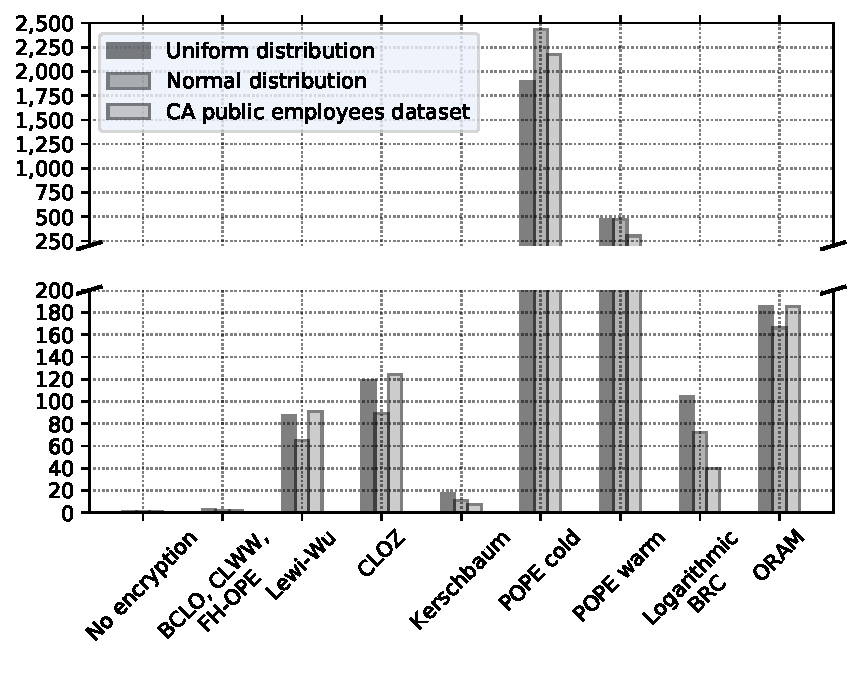
\includegraphics[width=0.6\textwidth]{protocol-charts-qios}
			\caption{
				Query stage number of I/O requests \\
				\hyperlink{frame:ore}{\beamerreturnbutton{Back to ORE}}
			}
		\end{figure}

	\end{frame}

	\begin{frame}[label={frame:appendix:oram}]

		\frametitle{Access pattern and ORAM}

		\justifying%

		\textbf{Access pattern} is a sequence of memory accesses \oramProgram{}, where each access consists of the memory \emph{location} $o$, read \oramRead{} or write \oramWrite{} \emph{operation} and the \emph{data} $d$ to be written.

		Oblivious RAM (ORAM) is a mechanism that hides the accesses pattern.
		More formally, \oram{} is a protocol between the client \client{} (who accesses) and the server \server{} (who stores), with a guarantee that the view of the server is indistinguishable for any two sequences of the same lengths.

		\begin{columns}[T]
			\column{0.475\textwidth}

				\[
					\begin{split}
						\abs{\oramProgram_1}					& = \abs{\oramProgram_2}							\\
						\textsc{View}_\server (\oramProgram_1)	& \cindist \textsc{View}_\server (\oramProgram_2)
					\end{split}
				\]

			\column{0.475\textwidth}

				\procedure[linenumbering]{\oram{} protocol}{
					\textbf{Client \client}											\>														\> \textbf{Server \server}	\\
					%
					\oramProgram{} = \left. (\oramRead, i, \bot) \right|_{i = 1}^5	\> 														\>							\\
					%
					\text{(client state)}											\> \sendmessageboth*[6em]{\algo{ORAM}{\oramProgram}}	\> \text{(server state)}	\\
					%
					\{ d_1, d_2, d_3, d_4, d_5 \}									\>														\>
				}

		\end{columns}

		\vspace*{1ex}

		For example: Square Root ORAM~\cite{oram-theory}, Hierarchical ORAM~\cite{oram-original}, Binary-Tree ORAM~\cite{binary-tree-oram}, Interleave Buffer Shuffle Square Root ORAM~\cite{shortest-path-oram}, TP-ORAM~\cite{tp-oram}, \textbf{Path-ORAM}~\cite{path-oram} and TaORAM~\cite{taostore}.
		\alert{ORAM incurs at least logarithmic overhead in the number of stored records.~\cite{oram-original}}
		\hyperlink{frame:epsolute-motivation}{\beamerreturnbutton{Back to \epsolute{}}}

	\end{frame}

	\begin{frame}[label={frame:appendix:dcpe}]

		\frametitle{Component: DCPE}

		\[
			\forall x, y, x \in \mathbb{X} : \algo{Dist}{x, y} < \algo{Dist}{x, z} - \beta \implies \algo{Dist}{f(x), f(y)} < \algo{Dist}{f(x), f(z)}
		\]

		\begin{itemize}
			\item<1->
				The scheme is by Riddhi Ghosal and Adam O'Neil
			\item<2->
				\textbf{Key generation}: sample at random length multiplier $s$ and seeds for samplers $K$
			\item<3->
				\textbf{Encrypt}: take input vector $x \in \RR^d$
				\begin{itemize}
					\item Sample nonce $n$
					\item Using nonce and seeds, sample a point $a$ on a $\beta$-radius $d$-dimensional ball
					\item New vector is extended times $s$ and points to $a$
				\end{itemize}
			\item<4->
				\textbf{Decrypt}: take encrypted vector $c \in \RR^d$ and nonce $n$
				\begin{itemize}
					\item Do same steps except \emph{shrink} times $s$ and \emph{remove} ball component
				\end{itemize}
		\end{itemize}

		\hyperlink{frame:knn}{\beamerreturnbutton{Back to \knn{}}}

	\end{frame}

	\begin{frame}[label={frame:appendix:trec-faiss}]

		\frametitle{Component: TREC dataset and FAISS~\cite{faiss}}

		\begin{itemize}
			\item<1->
				Dataset is 8.8M documents represented as vectors of 768 dimensions \\
				\begin{small}
					Thanks Hamed Zamani for the dataset
				\end{small}

			\item<2->
				Query is a 768-dimensional vector asking for $k = 1000$ closest (inner product) documents

			\item<3->
				% cspell:disable-next-lin
				Original document set is a \textbf{T}ext \textbf{RE}trieval \textbf{C}onference (TREC) test collection \\
				\begin{small}
					set of documents, set of topics (questions), and corresponding set of relevance judgments (right answers)
				\end{small}

			\item<4->
				FAISS~\cite{faiss}: GPU-enabled library for efficient similarity search and clustering of dense vectors
				\begin{small}
					Developed and maintained by Facebook AI
				\end{small}

			\item<5->
				General algorithm: for different $\beta$
				\begin{itemize}
					\item Encrypt dataset with $\beta$
					\item Encrypt queryset with $\beta$
					\item Run queries with FAISS
					\item Generate TREC metrics (using relevance judgments)
				\end{itemize}

		\end{itemize}

		\hyperlink{frame:knn}{\beamerreturnbutton{Back to \knn{}}}

	\end{frame}

	\begin{frame}[label={frame:appendix:knn-plot}]

		\frametitle{Intermediate results}

		\begin{figure}[h]
			\centering
			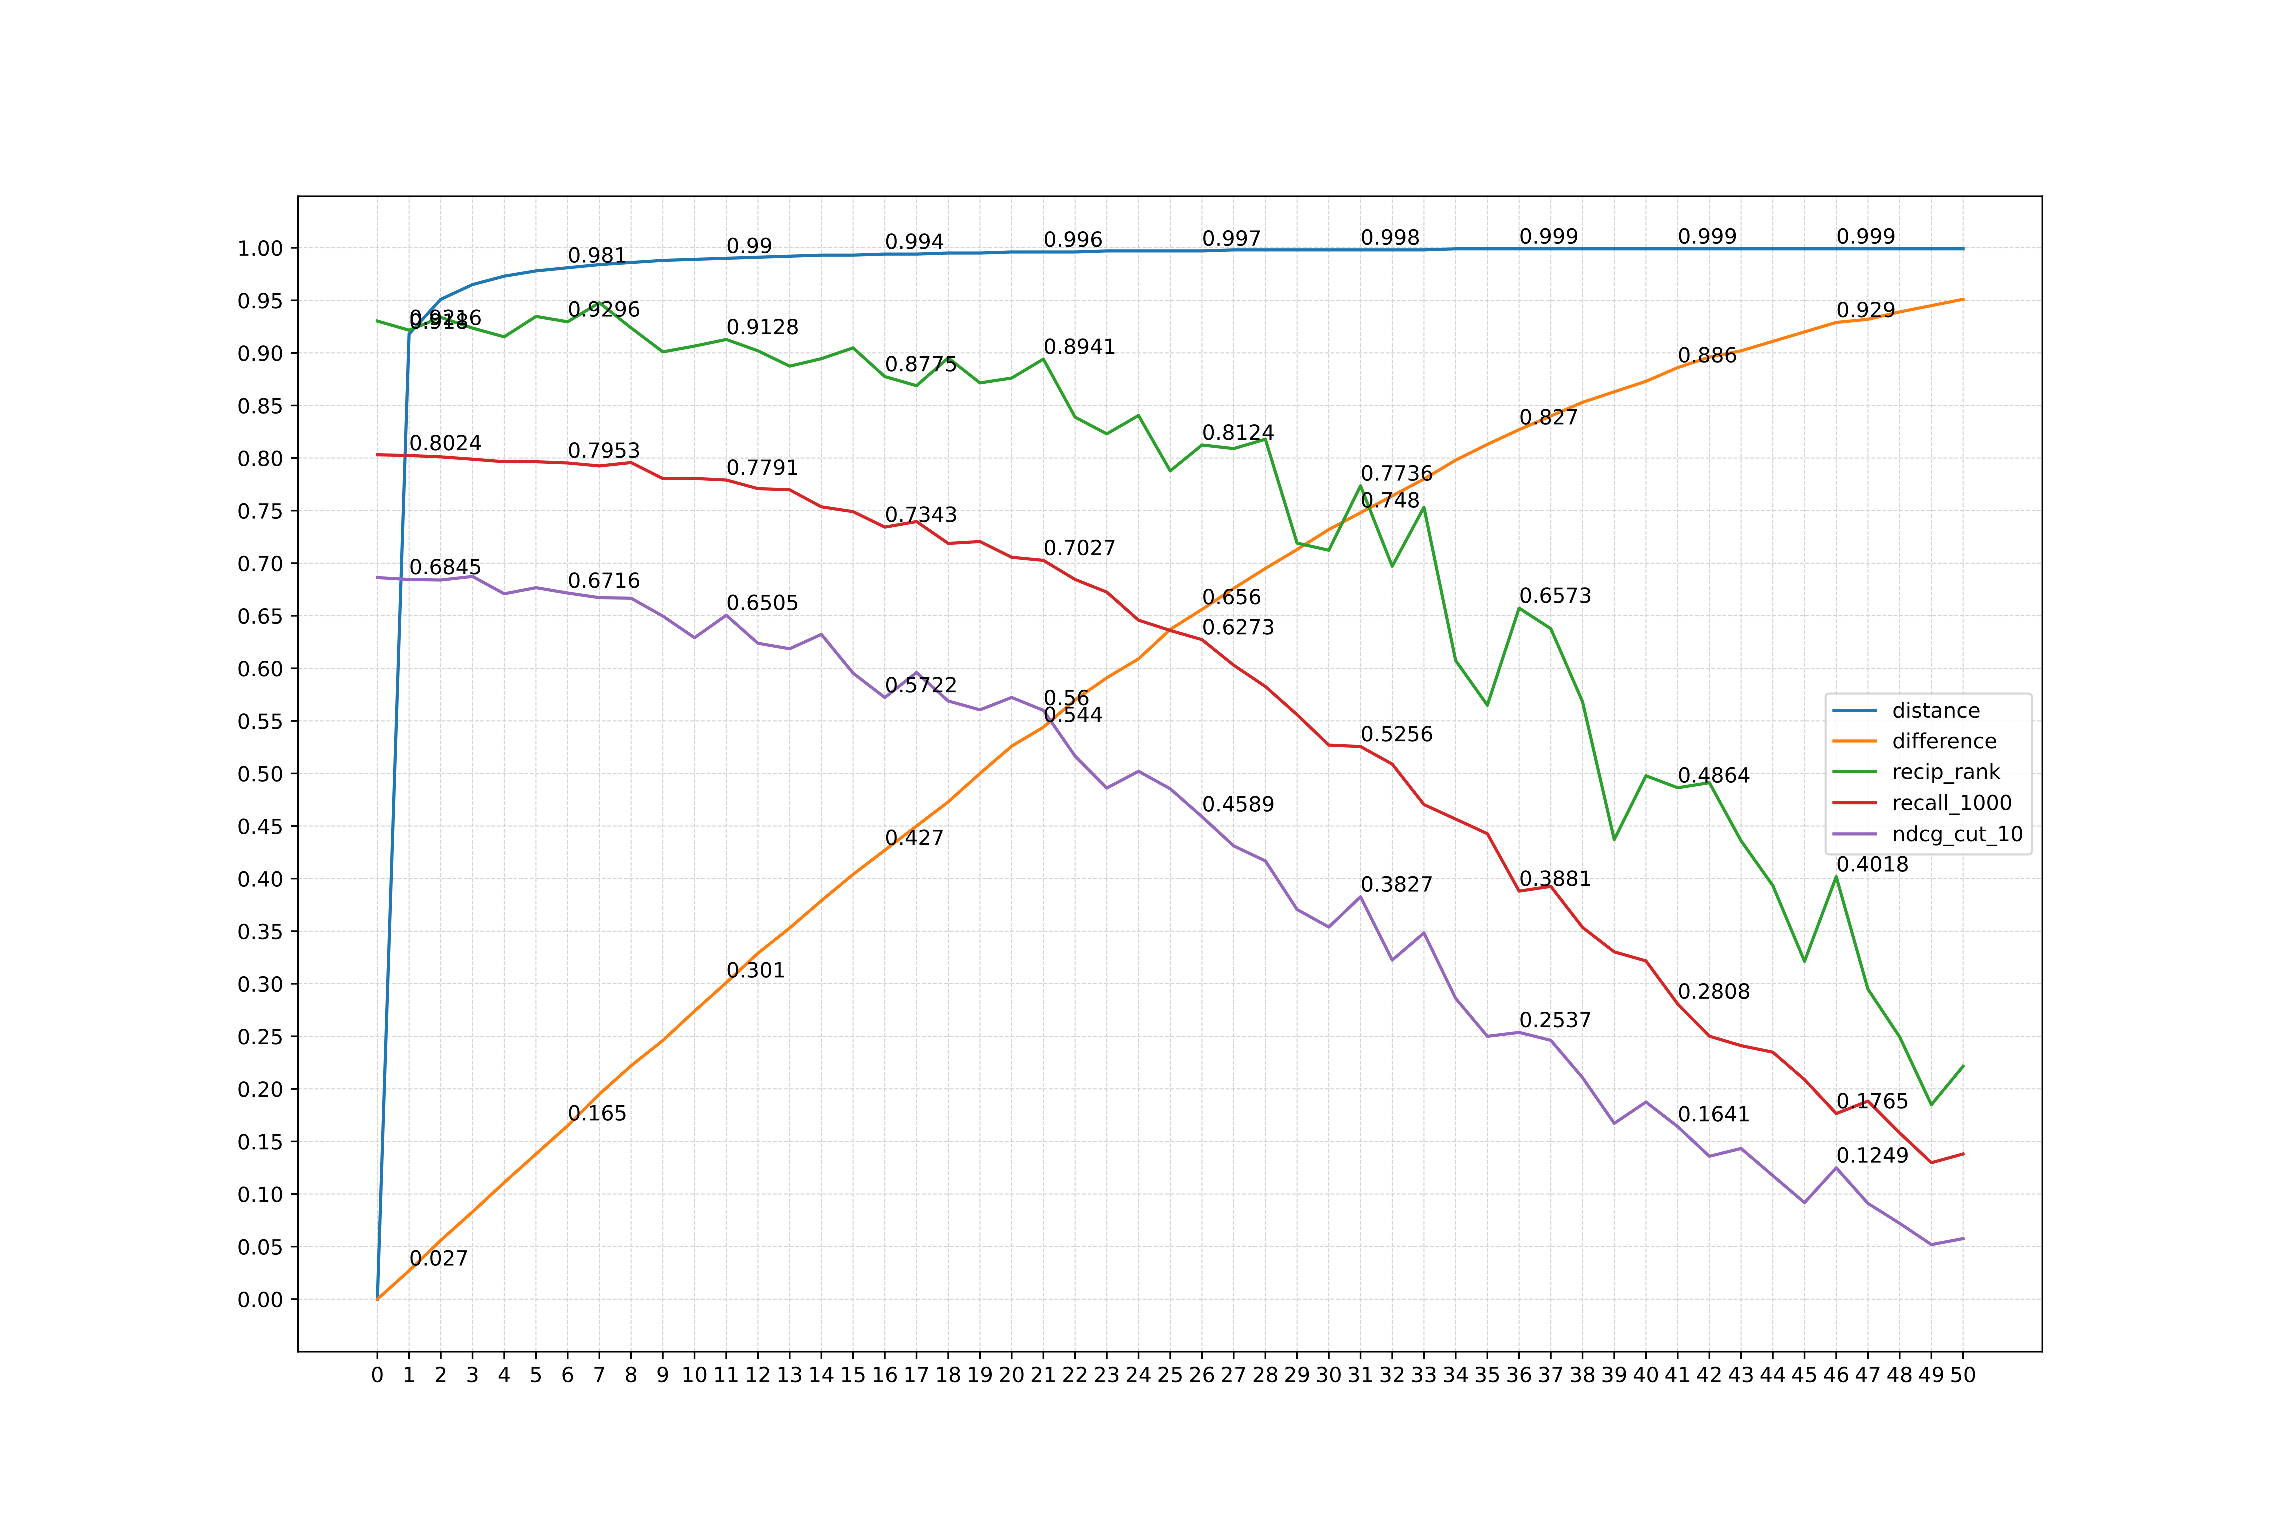
\includegraphics[trim=60 60 60 60,clip,width=0.75\textwidth]{knn}
			\caption{
				TREC metrics, result set distance and difference, for running \knn{} search for $\beta \in \{ 0, 1, \ldots , 50 \} $ \\
				\hyperlink{frame:knn}{\beamerreturnbutton{Back to \knn{}}}
			}
		\end{figure}

	\end{frame}

	\begin{frame}[label={frame:appendix:joins-detailed}]

		\frametitle{Oblivious \texttt{JOIN}s detailed algorithm}

		\begin{itemize}
			\item<1->
				Construct list $L$ of the form $(k, n_1, \hat{n_1}, n_2, \hat{n_2})$, with an element per distinct key plus noise \\
				\begin{small}
					$k$ is a join key, $n$ and $\hat{n}$ are real and $\widehat{\text{noisy}}$ numbers of records with that key in corresponding input table \\
					Noise sampled to a hierarchical sanitizer from a Laplacian distribution
				\end{small}

			\item<2->
				Client \user{} sends sorted $L$ and hierarchical sanitizer over noise counts to the server \server{} \\
				\begin{small}
					Similar to \epsolute{}, adversary does not learn much from noisy counts
				\end{small}

			\item<3->
				Server $\server{}$ partitions $L$ by $k$, so that partition size ($\hat{n_1} + \hat{n_2}$) is bounded and uniform \\
				\begin{small}
					Resulting mapping from keys to partitions $\mathcal{M}(k) = i$ can be proven DP
				\end{small}

			\item<4->
				Consolidate sparse keys: ensure that each \emph{bin} corresponds to at least $U$ real keys \\
				\begin{small}
					\emph{Bin} is collection of tuples for which we will do cross product join
				\end{small}

			\item<5->
				Obliviously move and pad each bin/partition with dummy records \\
				\begin{small}
					Within each bin the data is sorted by input tables
				\end{small}

			\item<6->
				For each bin, \textbf{do cartesian product}

		\end{itemize}

		\hyperlink{frame:oblivious-joins}{\beamerreturnbutton{Back to Oblivious Joins}}

	\end{frame}
